\documentclass{article}
\usepackage[T1]{fontenc}
\usepackage{microtype,graphicx,booktabs,amsmath,hyperref}
\usepackage[accepted]{mlsys2025}
\makeatletter
\renewcommand{\Notice@String}{Independent study artifact prepared with Codex. Not a conference acceptance or course submission.}
\gdef\mlsyscorrespondingauthor@text{not applicable; learner identity not supplied}
\makeatother
\mlsystitlerunning{KV Cache Granularity on CPU}
\begin{document}
\twocolumn[
\mlsystitle{KV Cache Granularity and Prefix Sharing on CPU}
\begin{mlsysauthorlist}
\mlsysauthor{AI-Assisted Independent Study}{self}
\end{mlsysauthorlist}
\mlsysaffiliation{self}{CMU 15-779 public-material self-study; no institutional affiliation or Andrew ID asserted}
\vskip 0.2in
\begin{abstract}
Paged K/V caches combine dynamic growth with opportunities to share prompt prefixes, but block granularity can erase sharing benefits when prefixes are short or poorly aligned. We implement a CPU allocator with prefix forks, reference counts and copy on write, and compare it with static reservation and dynamic concatenation. Across five synthetic workloads, three seeds and six block sizes, all 210 configuration rows match a dense attention reference; 1,470 timed executions preserve raw samples. For a 31-token common prefix, blocks of 4 retain 29 KiB of active K/V slots, whereas blocks of 32 retain 112 KiB and share no complete prefix block after divergence. The Python paged implementation remains slower than the dense baselines, and its active-slot savings do not shrink its preallocated pool. These results characterize granularity and implementation overhead, with no GPU, full-model throughput or peak-memory claim.
\end{abstract}
]
\printAffiliationsAndNotice{}

\section{Introduction}
Autoregressive serving retains keys and values from earlier tokens. Request lengths are not generally known in advance, and many requests may begin with the same system prompt or application context. Maximum-length reservation wastes space on shorter requests; repeated concatenation keeps only the required logical length but moves old values. PagedAttention addresses storage through block tables and a compatible attention kernel \citep{kwon2023}. SGLang additionally organizes reusable prefixes with RadixAttention and cache-aware execution \citep{zheng2024}.

This project asks a narrower question that can be investigated without a GPU: how do block size and prefix alignment affect retained slots and copying under controlled cache semantics? It contributes an independently written CPU allocator, a checked workload harness, a simple accounting model and preserved measurements. It is an exploratory systems study rather than a new paging algorithm. Separate course CUDA checks subsequently ran on an authorized GPU host; they are outside this CPU cache dataset.

\section{Problem and Scope}
Let R requests retain lengths $L_i$, share an identical prefix of length P, and use block size B. K and V each have width 16 and float64 elements, so a paired token slot is $s=256$ bytes. All requests retain their caches until the workload ends; every request appends at least one token beyond the shared prefix. Queries and K/V are fixed synthetic tensors. Identical prefix tensors represent valid reuse by construction. We do not infer reuse from text, run tokenization, or model arbitrary contextual equality.

\textbf{RQ1} examines retained slots as B and P vary. \textbf{RQ2} compares old-slot movement from concatenation with partial-page copy on write. \textbf{RQ3} measures the complete CPU cache path and distinguishes it from GPU kernel speed or service throughput. The experiment excludes arrival/admission scheduling, model projections, multilayer attention, sampling and language quality. A separate course lab demonstrates continuous batching with synthetic costs; those scheduling numbers are not mixed into this project's measurements.

\section{Related Work}
\textbf{PagedAttention.} \citet{kwon2023} map logical KV blocks to physical blocks and implement attention that directly follows the mapping. Reference counts and copy on write support multiple generation branches. We adopt these published storage concepts, but use CPU tensors and a gather before attention. Consequently, our runtime results are not a reproduction of vLLM or its kernel.

\textbf{SGLang.} \citet{zheng2024} combine a structured language with runtime optimizations including RadixAttention, prefix-aware execution and constrained decoding. Our known-prefix forks isolate storage granularity, without their radix-tree matching, LRU eviction or structured-program runtime. Knowing a prefix in advance avoids matching cost and makes reuse easier than general online serving.

\textbf{Attention and caching.} Transformer attention \citep{vaswani2017} motivates retained K/V. FlashAttention \citep{dao2022} reduces intermediate storage and data movement using tiled exact attention. Its online-softmax kernel optimizations solve a different problem from where persistent K/V pages live; our dense gather path implements neither GPU technique.

\section{System Overview}
Figure~\ref{fig:overview} separates input generation, storage policies and common numerical validation. All project code is original to this workspace. PyTorch supplies tensor allocation, indexing, concatenation, matrix-vector operations and softmax. Published paging/COW concepts and the official MLSys 2025 template are adopted and disclosed. No source implementation from vLLM or SGLang is imported.

\begin{figure*}[t]
\centering
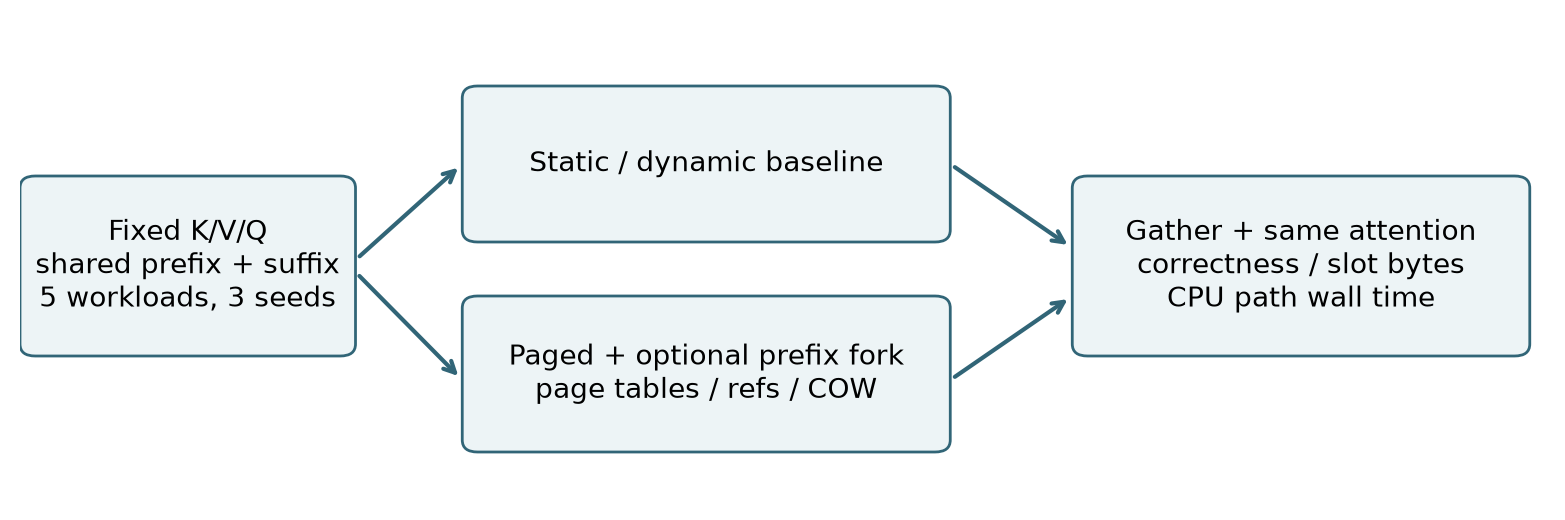
\includegraphics[width=\textwidth]{figures/architecture.png}
\caption{Implemented components. Fixed input generation and the dense reference are outside timing. The timed path includes policy allocation, prompt insertion, prefix forks where applicable, appends, gather, attention, output stacking and metric construction.}
\label{fig:overview}
\end{figure*}

The paged allocator preallocates paired K/V tensors, a free-page list, reference counts, per-sequence tables and logical lengths. Starting a sequence creates an empty table. Forking copies a table prefix and increments references, without copying K/V values. Appending allocates a new block at a boundary. If the append falls inside a shared partial page, it allocates a replacement, copies only the live prefix and decrements the old reference. Release returns a page only when the final reference disappears. Allocation failure occurs before changing existing sequence state.

\section{Method and Accounting}
\subsection{Storage Policies}
\textbf{Static} reserves a uniform maximum final length for every request. This is an explicit maximum-reservation baseline, not an optimized arena allocator. \textbf{Dynamic} clones each prompt and appends each decode token with \texttt{torch.cat}. \textbf{Paged} stores requests independently. \textbf{Shared} forks the supplied common prefix, then independently appends suffix/decode tokens. Paged variants gather contiguous K/V before applying the same attention expression as the baselines.

All requests are kept alive through the end, so retained length and the number of active physical pages are monotone. This enables final active-page bytes to describe maximum active-page occupancy for this specific workload. It does not measure transient peak allocation. We distinguish active-page bytes, full pool-tensor bytes and logical token references; Python objects, temporary gather/cat results, scores, inputs and allocator overhead are excluded from these storage counters.

\subsection{A Checkable Granularity Model}
Independent paging uses
\begin{equation}
S_{\mathrm{page}}=B\sum_{i=1}^{R}\left\lceil L_i/B\right\rceil
\end{equation}
paired slots. After every branch diverges, only complete prefix blocks remain shared, giving
\begin{equation}
S_{\mathrm{share}}=S_{\mathrm{page}}-(R-1)B\left\lfloor P/B\right\rfloor.
\label{eq:sharing}
\end{equation}
The partial-prefix boundary is copied for all but one branch, so old-slot copy count is
\begin{equation}
M_{\mathrm{COW}}=(R-1)(P\bmod B).
\end{equation}
These formulas assume exactly the supplied common prefix, all requests diverge, no eviction and this reference-counted COW policy. They do not describe arbitrary retained radix-cache entries or unfinished branches.

With prompt length $p_i$ and $d_i$ appends, dynamic concatenation moves
\begin{equation}
M_{\mathrm{cat}}=\sum_i\left(d_i p_i+d_i(d_i-1)/2\right)
\end{equation}
old paired slots. New-token writes, initial prompt writes, gather traffic, CPU caches and physical DRAM transactions are not included. Multiplying this logical movement count by s gives algorithmic bytes copied, not measured memory-bus traffic.

\subsection{Correctness}
Every decode output is compared against attention over the complete retained dense prefix. The baseline recomputes reference output independently of the tested storage. Float64 tolerance is $10^{-12}$ absolute and relative; observed maximum error is zero for all recorded configurations. Tests separately validate output/gradient identities elsewhere in the course, while project tests cover block boundaries and Equations~\ref{eq:sharing}--3. The allocator's randomized histories compare every live sequence with independent storage after fork, truncated-prefix fork, append and release. Both new-page and COW out-of-memory paths preserve prior state. This is strong finite testing of the implementation, not a proof for all programs or floating-point inputs.

\section{Evaluation}
\subsection{Setup and Reproducibility}
Experiments ran on macOS 26.6.2 arm64, Python 3.11.15, PyTorch 2.14.1, with one CPU thread and float64 tensors. No MPS or CUDA operations execute. Five workload families contain P=0,3,31,32,63 shared-prefix tokens. Base prompt lengths equal P except independent requests use 31. Eight requests add suffix lengths $[0,1,3,7]$ twice and decode lengths $[1,2,4,8]$ twice. Widths are 16 for both K and V. No external dataset is used.

Each family runs seeds 41,42,43. Four policy types include six sizes B=2,4,8,16,32,64 for each paged variant, yielding 14 configurations per family/seed and 210 rows total. Each configuration warms up once, then runs seven times. Policy order is shuffled each repetition. Input generation and correctness assertions are excluded; complete policy execution is timed with a monotonic wall clock. Figures show the median of three per-seed medians; raw samples remain available. This descriptive aggregation is not an independent-run confidence interval. Background activity and allocator effects are not fully isolated.

\begin{table*}[t]
\caption{Retained K/V slots in KiB (1 KiB=1024 bytes). Shared columns use the indicated B. These are active slots, not RSS or pool shrinkage. Values are deterministic across seeds.}
\label{tab:storage}
\centering
\begin{tabular}{lrrrrr}
\toprule
Workload & Static & Dynamic & Shared B=4 & Shared B=32 & Shared B=64\\
\midrule
independent & 92 & 75 & 78 & 112 & 128 \\
shared\_3 & 36 & 19 & 22 & 64 & 128 \\
shared\_31 & 92 & 75 & 29 & 112 & 128 \\
shared\_32 & 94 & 77 & 24 & 72 & 128 \\
shared\_63 & 156 & 139 & 37 & 120 & 224 \\
\bottomrule
\end{tabular}

\end{table*}

\begin{figure*}[t]
\centering
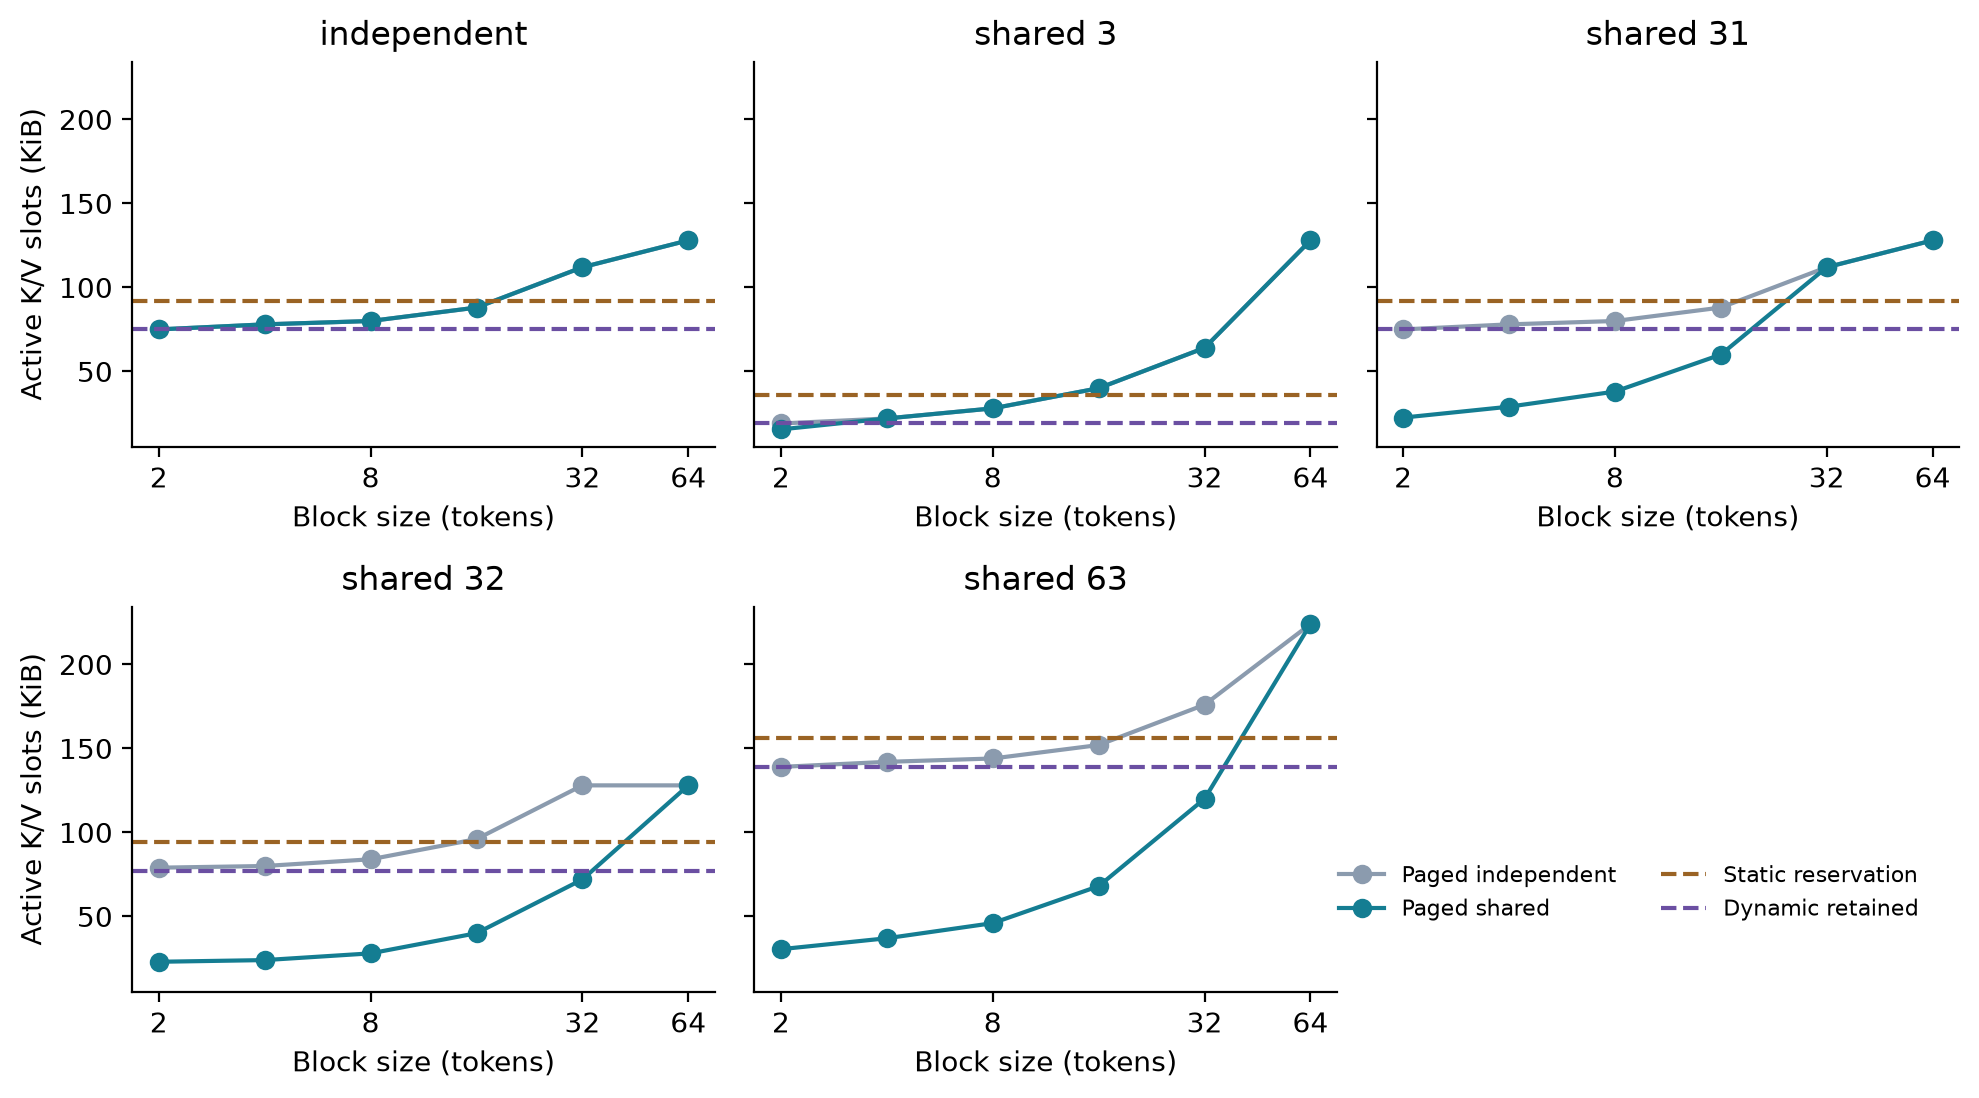
\includegraphics[width=\textwidth]{figures/storage.png}
\caption{Granularity sweep. Short or misaligned prefixes can lose full-block reuse; larger blocks also increase tail waste. The independent workload deliberately has no reusable prefix.}
\label{fig:storage}
\end{figure*}

\subsection{Storage and Prefix Alignment}
Table~\ref{tab:storage} and Figure~\ref{fig:storage} support a specific conclusion: reuse depends on complete prefix blocks after divergence, not merely the presence of identical prompt tokens. For P=31, B=4 uses 29 KiB versus 78 KiB for independent paging and 75 KiB for dynamic retention. B=32 has no complete common block, retains 112 KiB and exceeds the 92 KiB static baseline. Thus paging alone need not save slots at a coarse granularity.

P=32 aligns with B=32 and retains 72 KiB versus 128 KiB for independent paging. Yet B=4 retains 24 KiB, because the much smaller per-request tails outweigh the reduction in metadata from large blocks. When P=3, B=4 likewise shares no complete prefix block after divergence. With B=64, that short workload retains 128 KiB despite only 19 KiB of logically required independent values. These examples expose a page-size effect rather than a universal best hardware block size.

\subsection{Copies, Metadata and Reserved Pools}
At P=31, B=4 copies 21 old paired slots, B=32 copies 217, and B=2 copies 7, exactly matching $(R-1)(P\bmod B)$. Dynamic concatenation copies 1,140 old slots in that workload. However, the paged path also gathers K/V for every attention call, so fewer COW copies alone do not imply less total data movement. Table-entry counts are recorded rather than converted into unreliable Python metadata-byte estimates.

The pool is sized to the complete independent-paging capacity and allocated identically for shared and unshared policies at a given B. At P=31/B=4, shared active storage is 29 KiB but its pool remains 78 KiB. Returning logical pages enables reuse within that pool; it does not return tensor backing memory to the operating system. Dynamic retained storage similarly excludes old/new allocation overlap during concatenation. No result is described as measured process peak memory.

\begin{figure*}[t]
\centering
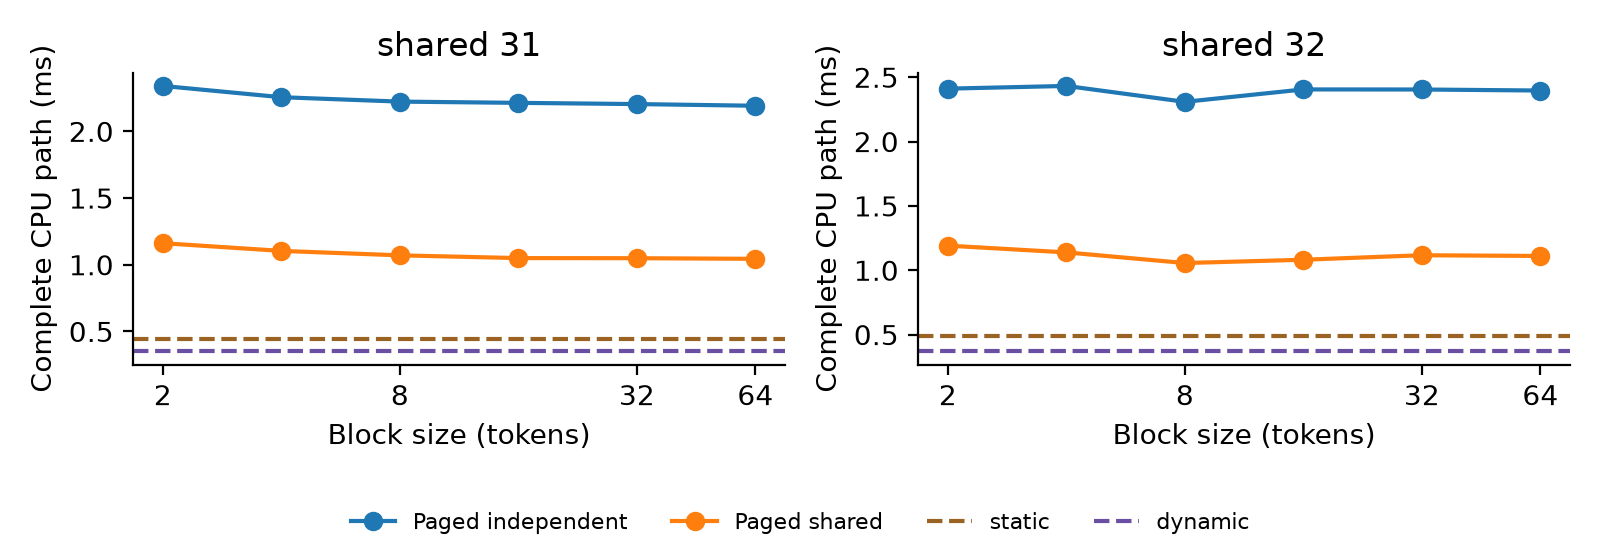
\includegraphics[width=0.85\textwidth]{figures/latency.png}
\caption{Complete CPU policy-path time, median of per-seed medians. Python per-token paging and materializing gathers make paged variants slower than the dense baselines. This is not GPU attention kernel latency.}
\label{fig:latency}
\end{figure*}

\subsection{Runtime Interpretation}
Figure~\ref{fig:latency} shows that prefix forks reduce setup work relative to independent paging, but both remain slower than the dense baselines. For P=31 in seed 41, dynamic takes approximately 0.35 ms, shared B=4 about 1.10 ms, and independent B=4 about 2.26 ms. These illustrative values are medians of seven complete-path repetitions; other seeds and full samples are preserved. An implementation that performs Python work per token and gathers the full context should not be expected to reproduce a fused paged GPU kernel. We report the adverse timing result rather than presenting active-slot reductions as acceleration.

\section{Limitations and Threats to Validity}
The controlled workload omits causal contextual projections, full models, user arrival processes, active-request admission, eviction, multiple layers/heads and tensor-parallel communication. Keeping completed requests alive simplifies accounting and differs from a serving system that immediately frees them. Known-prefix forks omit radix matching and cache-identity checks. Real reuse must account for model weights/version, tokenization, positions and full causal prefix, not matching suffix strings.

CPU timings include setup and Python metrics, not isolated attention or append microbenchmarks. Small matrices and one thread do not capture GPU occupancy, launch costs or memory-bandwidth saturation. The six sizes are a study grid, not a hardware tuning recommendation. Input K/V are finite random float64 values; quantization, low-precision kernels and generation quality are not evaluated. The study supports its storage formulas and observed implementation costs only.

\section{Conclusion}
Under a controlled CPU cache workload, complete shared prefix blocks reduce active K/V slots, while partial-page divergence requires copying and coarse blocks can exceed even static reservation. Separating active slots from the reserved pool prevents false peak-memory claims. All recorded outputs match the dense reference, but the Python paged implementation is slower than dense baselines. The reusable contribution is a checked allocator, explicit granularity/copy model and transparent measurements for further implementation work, not evidence of GPU or end-to-end serving speedup.

\section*{Artifact and Authorship Record}
Code, tests, workload seeds, raw timings, environment and SHA256 source hashes are saved locally. Run \texttt{course/project/run\_experiments.py}, followed by \texttt{analyze\_results.py}. This report, code and narration were prepared with Codex for independent study. Learner/team identity and Andrew IDs were not provided; personal mastery, classroom participation and formal submissions are not asserted. Native CUDA and Triton/SDPA checks are separately archived and do not turn this cache study into a GPU result. The official MLSys 2025 style is used with a self-study notice; its visibility option is not a claim of conference acceptance.

\clearpage
\bibliographystyle{mlsys2025}
\bibliography{references}
\end{document}
